\documentclass[11pt]{article}
\usepackage[margin=1in]{geometry}
\usepackage{booktabs}
\usepackage{graphicx}
\usepackage{hyperref}
\usepackage{microtype}
\usepackage{amsmath}
\usepackage{enumitem}

\title{A Reproducible Baseline for Grokking in Modular Addition}
\author{Igor Rybakoff}
\date{}

\begin{document}
\maketitle

\begin{abstract}
Grokking is a delayed transition from memorization to generalization in which a neural network attains high training performance long before comparable held-out performance. We present a reproducibility-focused single-run baseline for grokking on modular addition, using a compact one-layer Transformer trained on $(a+b)\bmod 113$. The frozen run uses a deterministic seed, a 30/70 train-validation split, full-batch AdamW, fixed evaluation thresholds, and 40{,}000 optimization steps. Training accuracy crosses 0.98 at step 200 while validation accuracy remains near chance; validation accuracy first crosses 0.985 at step 25{,}600 and remains above threshold for ten consecutive logged evaluations by step 26{,}500. Final training and validation accuracy both reach 1.0. In addition to the training time series, the released evidence package contains five SHA-256-verified PyTorch checkpoints, checkpoint replay reports, configuration metadata, and a generated training curve. The contribution is not a new mechanistic theory of grokking, but an auditable baseline that separates measured artifacts from interpretation and states explicit reproducibility boundaries.
\end{abstract}

\section{Introduction}
Grokking was introduced as a striking regime in which generalization occurs well after a model has already fit its training data \cite{power2022grokking}. Modular arithmetic provides a compact setting in which memorization, generalization, optimization, and representation learning can be studied under controlled conditions. Subsequent work has extended grokking beyond algorithmic data \cite{liu2022omnigrok}, analyzed its internal mechanisms with mechanistic interpretability \cite{nanda2023progress}, and examined the role of the embedding layer and optimization dynamics \cite{alquboj2025embedding}.

This paper takes a deliberately narrower position. We do not propose a new scientific definition or causal explanation of grokking. Instead, we ask whether one grokking run can be packaged so that its claims are directly inspectable through frozen metrics, explicit event rules, cryptographic integrity checks, and checkpoint replay.

The resulting artifact, Grokking Lab, is an open-source PyTorch package built around a single frozen run. Its guiding reporting rule is simple: measured quantities come from the training and verification pipeline; language-model-assisted interpretation, if used, is downstream of those measurements and does not create them.

\section{Related Work}
Power et al.\ \cite{power2022grokking} demonstrated delayed generalization on small algorithmic datasets, including modular arithmetic, and showed that generalization can arise long after overfitting. Liu, Michaud, and Tegmark \cite{liu2022omnigrok} studied grokking through training and test loss geometry and showed that similar behavior can be induced beyond algorithmic tasks. Nanda et al.\ \cite{nanda2023progress} reverse-engineered small Transformers trained on modular addition and identified continuous progress measures underlying the apparently abrupt transition. More recently, AlquBoj et al.\ \cite{alquboj2025embedding} investigated embedding-layer dynamics and bilinear coupling as mechanisms that affect grokking behavior.

Our contribution is complementary. Rather than advancing a mechanistic hypothesis, we provide a compact evidence package for one controlled run, with explicit milestone thresholds, replayable checkpoints, integrity metadata, and a documented boundary between what is reproduced and what is merely reconstructed from historical artifacts.

\section{Experimental Setup}
The task is modular addition:
\[
y=(a+b)\bmod 113.
\]
Each input is tokenized as \texttt{[a, b, EQUALS]} with context length 3. The model predicts the result at the final position. The complete modular-addition table is deterministically partitioned into 30\% training and 70\% validation data using seed 42.

\begin{table}[h]
\centering
\caption{Frozen experimental configuration.}
\begin{tabular}{ll}
\toprule
Task & $(a+b)\bmod 113$ \\
Train / validation split & 30\% / 70\% \\
Seed & 42 \\
Architecture & one-layer Transformer \\
Model width & $d_{\mathrm{model}}=128$ \\
Attention heads & 4 \\
MLP width & $d_{\mathrm{mlp}}=512$ \\
Normalization & none \\
Dropout & 0.0 \\
Activation & ReLU \\
Attention & causal \\
Optimizer & full-batch AdamW \\
Learning rate & 0.001 \\
Weight decay & 1.0 \\
Training steps & 40{,}000 \\
Logging interval & 100 steps \\
\bottomrule
\end{tabular}
\end{table}

The frozen manifest records CPU execution with Python 3.14.3, PyTorch 2.13.0, and NumPy 2.5.1. These environment values describe the historical run; they are not claimed to guarantee bitwise-identical retraining on other systems.

\section{Milestone Detection Policy}
To avoid retroactively choosing favorable transition points, milestones are computed by a deterministic policy over the logged time series.

Let $A_{\mathrm{train}}(t)$ and $A_{\mathrm{val}}(t)$ denote training and validation accuracy at logged step $t$.

\begin{itemize}[leftmargin=*]
    \item \textbf{Memorization step:} first logged step with $A_{\mathrm{train}}\ge 0.98$.
    \item \textbf{Generalization candidate:} first logged step with $A_{\mathrm{val}}\ge 0.985$.
    \item \textbf{Stable plateau:} first step completing 10 consecutive logged evaluations with $A_{\mathrm{val}}\ge 0.985$.
\end{itemize}

Because metrics are logged every 100 steps, these milestones are interval-limited observations, not exact continuous-time transition points. The repository label \texttt{GROKKING\_CONFIRMED} means only that the stable-plateau rule is satisfied under this event policy.

\section{Results}
The frozen run contains 401 measured records from step 0 through step 40{,}000. Table~\ref{tab:milestones} summarizes the replay-verified checkpoints.

\begin{table}[h]
\centering
\caption{Replay-verified milestone checkpoints.}
\label{tab:milestones}
\begin{tabular}{rrrrr}
\toprule
Step & Train acc. & Val. acc. & Train loss & Val. loss \\
\midrule
0 & 0.00940 & 0.00940 & 5.04193 & 5.03410 \\
200 & 0.99843 & 0.00045 & 0.06921 & 19.56679 \\
25{,}600 & 1.00000 & 0.99776 & 0.00479 & 0.03232 \\
26{,}500 & 1.00000 & 1.00000 & 0.00186 & 0.00274 \\
40{,}000 & 1.00000 & 1.00000 & $1.86\times10^{-6}$ & $2.59\times10^{-6}$ \\
\bottomrule
\end{tabular}
\end{table}

At step 200, training accuracy is already approximately 0.9984 while validation accuracy is approximately 0.00045. The large separation between training and validation performance persists for most of training. Validation accuracy first exceeds the repository's 0.985 generalization threshold at step 25{,}600 and satisfies the ten-check stability criterion at step 26{,}500. Final training and validation accuracy are both 1.0.

\begin{figure}[h]
\centering
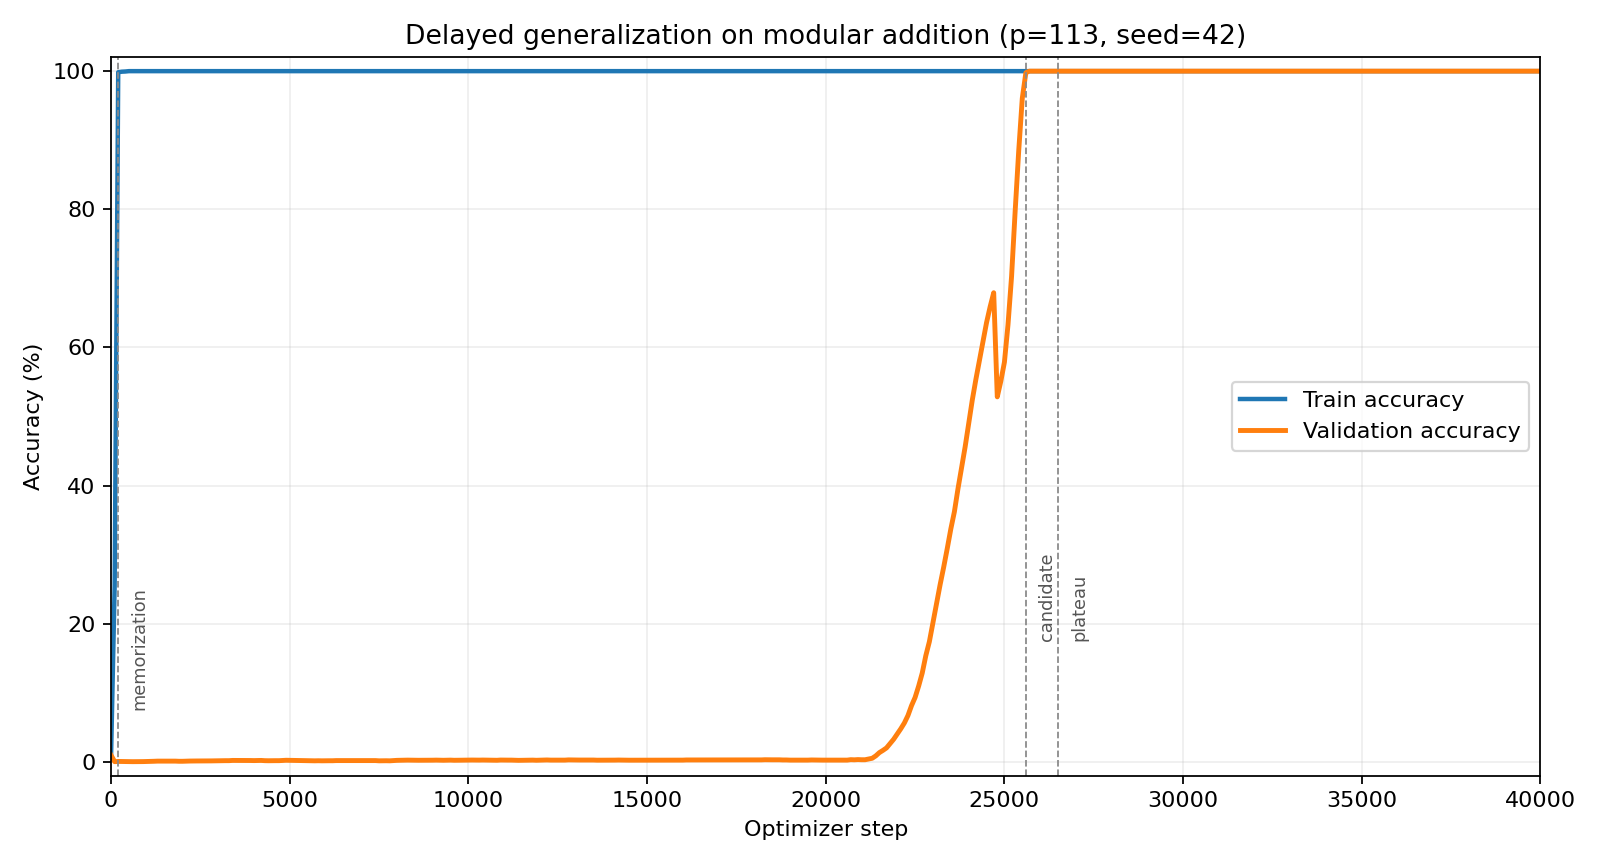
\includegraphics[width=\linewidth]{../artifacts/p113_seed42_40k/plots/grokking_curve.png}
\caption{Measured training and validation accuracy from the frozen 40{,}000-step run. The plot is generated directly from the stored time series without smoothing or synthetic points.}
\label{fig:grokking}
\end{figure}

This pattern is behaviorally consistent with delayed generalization: near-complete memorization occurs early, while held-out performance improves much later.

\section{Reproducibility and Provenance}
The public release separates four levels of verification.

\paragraph{Artifact integrity.}
The evidence package includes SHA-256 checksums for published artifacts and verifies the expected 0--40{,}000 step sequence at 100-step intervals.

\paragraph{Checkpoint replay.}
Five PyTorch state-dict checkpoints are published for initialization, memorization, generalization candidate, plateau, and final state. Replay reconstructs the deterministic dataset split, performs new forward passes, and compares losses and accuracies against the frozen replay report. The published manifest reports a replay maximum absolute metric difference of 0.0 for these checkpoints.

\paragraph{Smoke training.}
A short PyTorch smoke test performs real forward, backward, and AdamW update steps and verifies that parameters change. It is a training-path test, not a grokking reproduction.

\paragraph{Optional long-run reproduction.}
A 40{,}000-step execution recipe is provided. Independent reruns are intended to be recorded separately rather than overwriting the historical evidence package.

The repository therefore distinguishes evidence integrity, functional replay compatibility, execution-path testing, and full retraining. These are related but not equivalent claims.

\section{Limitations}
This work intentionally makes a narrow claim.

First, the evidence package contains one seed. It does not establish robustness across seeds, moduli, architectures, optimizers, train fractions, or scales. Second, modular addition is a synthetic complete table and should not be treated as a proxy for language or multimodal generalization. Third, milestone steps depend on explicit thresholds and the 100-step logging cadence. Fourth, the behavioral transition does not identify the causal circuit or optimization mechanism responsible for grokking.

Most importantly, the original historical run did not preserve a source-code hash or an explicit split-index file. Public v0.1 therefore does not claim byte identity with the original internal training script. The released implementation follows the recorded architecture contract, reconstructs the deterministic split rule, and uses checkpoint replay as its compatibility gate.

Checksums provide integrity control for the published package; they do not constitute independent third-party attestation.

\section{Discussion}
The value of this baseline is methodological rather than state-of-the-art performance. Grokking experiments are unusually sensitive to training duration, regularization, initialization, architecture details, and evaluation definitions. A result can therefore be difficult to compare when event definitions or artifacts are missing.

The present package makes the following items explicit: the complete model contract, train-validation split rule, optimizer configuration, event thresholds, full logged time series, selected checkpoints, replay results, integrity hashes, and known provenance gaps.

This structure creates a stable baseline for future controlled interventions. A useful next step is a multi-seed study in which one variable is changed at a time while preserving the same reporting and artifact policy.

\section{Conclusion}
We present a reproducibility-focused baseline for grokking in modular addition. In the frozen seed-42 run, a one-layer Transformer memorizes the training subset by step 200 while validation performance remains near chance, then transitions to near-perfect validation accuracy around step 25{,}600 and reaches a stable plateau by step 26{,}500.

The central contribution is not a new theory of grokking, but a compact auditable evidence package: fixed configuration, deterministic event detection, measured time series, SHA-256-verified checkpoints, functional replay, and explicit reproducibility limits.

Code and artifacts are available at:
\url{https://github.com/IgorRybakoff/grokking-lab}

\bibliographystyle{plain}
\bibliography{references}

\appendix
\section{Artifact Map}
The public evidence base contains multiple independent long runs and supporting controls. The three principal $p=113$ runs are:

\begin{center}
\begin{tabular}{lll}
\toprule
Seed & Experiment ID & Final status \\
\midrule
42 & \texttt{exp\_1785360132042\_p113} & \texttt{GROKKING\_CONFIRMED} \\
43 & \texttt{exp\_1785406284582\_p113} & \texttt{GROKKING\_CONFIRMED} \\
44 & \texttt{exp\_p113\_seed44\_research\_v04} & \texttt{GROKKING\_CONFIRMED} \\
\bottomrule
\end{tabular}
\end{center}

For the seed-42 public package, the core artifacts include:
\begin{itemize}[leftmargin=*]
\item \path{config.json}
\item \path{experiment_manifest.json}
\item \path{training_timeseries.json}
\item \path{grokking_event_detection.json}
\item \path{checkpoint_replay_report.json}
\item \path{SHA256SUMS}
\item \path{artifact_index.json}
\end{itemize}

The later seed-44 publication protocol additionally preserves:
\begin{itemize}[leftmargin=*]
\item \path{dataset_split.json}
\item \path{environment_lock.json}
\item \path{source_hash_manifest.json}
\item configuration, source, split, and environment hashes bound into checkpoint metadata.
\end{itemize}

\section{Milestone Summary}
\begin{center}
\begin{tabular}{rrrr}
\toprule
Seed & Memorization & Candidate & Plateau \\
\midrule
42 & 200 & 25{,}600 & 26{,}500 \\
43 & 302 & 32{,}300 & 33{,}200 \\
44 & 416 & 23{,}000 & 23{,}900 \\
\bottomrule
\end{tabular}
\end{center}

For seeds 43 and 44, memorization is detected at optimizer-step resolution. The seed-42 historical package records this event at the older 100-step logging resolution.

\section{Checkpoint Roles}
Each principal run preserves semantically distinct checkpoints for initialization, memorization, first generalization-threshold crossing, stable plateau, and final model state. Checkpoint replay is used as a functional compatibility gate rather than assuming that file integrity alone proves scientific correctness.

\section{Negative Controls}
Small-modulus runs at $p=11$ were used as boundary and negative controls. They include memorization-only and partial-generalization outcomes and therefore demonstrate that the classifier does not automatically promote every completed run to \texttt{GROKKING\_CONFIRMED}.

\section{Provenance Boundary}
The provenance protocol evolved during the project. The earlier seed-42 and seed-43 runs preserve real PyTorch artifacts, measured timeseries, and replayable checkpoints. The later seed-44 run uses publication protocol v0.4 and additionally records source hashes, an environment lock, and exact dataset split indices.

The seed-44 source-freeze manifest records SHA-256 hashes for the training and audit code and reports no missing source files. The environment lock records Python 3.14.3, PyTorch 2.13.0, NumPy 2.5.1, macOS arm64, CPU execution, and float32 arithmetic.

The source-freeze metadata also records that Git dirty-state detection was unavailable because the experiment directory itself was not a Git repository. Accordingly, the source-hash manifest is treated as the relevant integrity record rather than a verified Git working-tree state.

\section{Reproduction Commands}
Artifact verification:
\begin{verbatim}
python scripts/verify_artifacts.py
\end{verbatim}
Checkpoint replay:
\begin{verbatim}
python scripts/replay_checkpoint.py \
  --checkpoint memorization_model_state.pt
python scripts/replay_checkpoint.py \
  --checkpoint final_model_state.pt
\end{verbatim}
Optional long-run reproduction:
\begin{verbatim}
python scripts/run_experiment.py \
  --config configs/p113_seed42_40k.json \
  --output runs/p113_seed42_40k
\end{verbatim}
Independent reruns should be preserved as distinct experiments rather than overwriting historical evidence.


\end{document}
